\section{BCE model}
\todo[inline]{Thomas M: indsæt model og forklar}
\begin{figure}[ht]
\centering
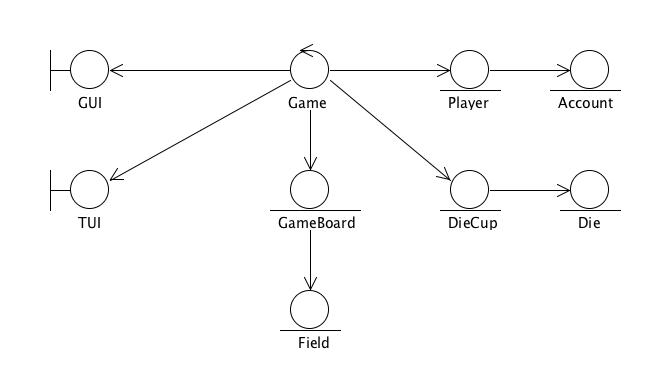
\includegraphics[scale=0.5]{BCE.jpg}
\caption[<Text for the list of figures>]{BCE Model}
\label{fig:figure 2}
\end{figure}
Vi har i denne del af CDIO opgaven ikke fået udleveret nogen BCE model.
\\
Vi har derfor udarbejdet et nyt diagram på baggrund af det fra vores CDIO del 1, da vi har genbrugt en del fra vores første program.
\\
Det vil sige at vi i denne model kun har tilføjet vores nye entitetsklasser. Det handler om entiteterne \textit{Account}, \textit{Field}, og \textit{GameBoard}. Vi har også lavet en ny boundary vi kalder \textit{Graphic}, som bearbejder beskeder til vores importerede \textit{GUI}.
\\
Som det fremgår af diagrammet, styrer controlleren \textit{Game} stadig spillet. Det vil sige at vores controller tildeler ansvaret ud til de nære klasser.
\\
\textit{Account} er en pengebeholdning der styres af \textit{Player} klassen. Vores controller har derfor kun brug for direkte kendskab til \textit{Player}.
\\\\
\textit{Field} holder styr på felterne i spillet, og vores \textit{Gameboard} holder styr på felterne. Vores \textit{Game} controller har dermed kendskab til felterne i spillet gennem vores \textit{Gameboard}.
\\


Ud fra disse informationer kan controlleren så sende besked til vores boundary's \textit{TUI} og \textit{Graphic}, som viser brugeren konsekvenserne i spillet grafisk og i tekst.